
\documentclass[preprint,12pt]{elsarticle}

\usepackage[spanish]{babel}
\usepackage{amssymb}
\usepackage{graphicx}
\usepackage{lineno}
\usepackage[utf8]{inputenc}
\usepackage{url}
\usepackage{color}
\usepackage{enumerate} 
\usepackage[hidelinks]{hyperref}


\begin{document}
	
	\begin{frontmatter}
		
		
		\title{\huge Sistema de Recomendación de Libros de Biblioteca}
		\author{Marlon Villegas Arando (2015053890)}
		\author{Lisbeth Espinoza Caso  (2011040667)}
		
		\address{Tacna, Perú}
		\address{2019}
		
		\begin{abstract}
			%% Text of abstract
			
The recommendation systems are part of an information filtering system, which present different types of topics or information items (movies, music, books, news, images, web pages, etc.) that are of interest to a user. particular. In this short article we will try to provide a general explanation about the different data models, such as Content Filtering and Collaborative Filtering.
Then we will apply these models in an example with the help of Colab, where we will filter data and show the results as well as their different graphs.
Then we will give some appreciations and conclusions of what was our Final Work.\\
		\end{abstract}
\end{frontmatter}
%%

	
	%%
	%\linenumbers
	
	%% main text
	\section{Resumen}
Los sistemas de recomendación forman parte de un sistema de filtrado de información, los cuales presentan distintos tipos de temas o ítems de información (películas, música, libros, noticias, imágenes, páginas web, etc.) que son del interés de un usuario en particular. En este breve artículo intentaremos brindar una explicación general acerca de los diferentes modelos de datos, tales como el Filtrado por Contenido y Filtrado Colaborativo.
Luego se aplicarán dichos modelos en un ejemplo con ayuda de Colab, donde filtraremos datos y mostraremos los resultados así como sus diferentes gráficas.
Luego daremos unas apreciaciones y conclusiones de lo que fue nuestro Trabajo Final.\\
	%%
	
	%%
	%\linenumbers
	
	%% main text

\section{Introduccion}

Todos hemos estado expuestos a los famosos “filtros colaborativos”: cuando estabas comprando online y automáticamente el sitio web te recomienda otro artículo similar, o cuando le diste “me gusta” a algo y de repente te empezaron a salir recomendaciones similares en una red social. Los sistemas de recomendación evalúan patrones de tu comportamiento y de miles de usuarios a la vez para emitir nuevas recomendaciones. Ésta es una de las aplicaciones más comunes de “Machine Learning”, porque te da la sensación de estar navegando en un sitio web programado únicamente para tí.

La mayoría de sistemas de recomendación de productos usan filtros colaborativos. Estamos en una era donde nosotros como usuarios generamos más información que nunca antes en la historia. Esta información es usada por los servicios que usamos a diario para darnos una experiencia mas personalizada.

Un claro ejemplo de esto es Netflix, ellos usan la información que nosotros generamos para hacernos recomendaciones y mostrarnos categorías y películas según nuestros gustos. Otro ejemplo es Amazon, que hace recomendaciones de productos que nos podrían interesar, basándose en los productos que ya compramos.

El filtro colaborativo es una técnica usada por los sistemas de recomendación, se basa en el hecho de que si dos personas X y Y en un mismo sistema tienen gustos similares, entonces recomendarle a la persona X cosas que le gusten a la persona Y será de gran relevancia, en contraste a simplemente darle una opción cualquiera.

Hay una variación de filtro colaborativo que se basa en comparar los items en vez de los usuarios para arrojar los items relacionados, de modo que si un usuario entra a ver un determinado item, le podemos recomendar otro.\\

\pagebreak
	%%
	
	%%
	%\linenumbers
	
	%% main text

\section{Marco Teorico}
 
\begin{enumerate}[3.1]
    \item Filtrado Contenido \\

El filtro de contenido web es una solución de software y/o hardware que tiene como finalidad actuar como un intermediario entre los accesos de los colaboradores a internet, posibilitando la aplicación de políticas definidas por la empresa.\\

Esto significa que el acceso a Internet deja de ser hecho directamente por el ordenador y pasa a ser realizado a través de la solución de filtrado de contenido web. Para el usuario esta transacción puede ser transparente, o mediante el uso de credenciales para el reconocimiento del usuario durante el primer intento de acceso a Internet. Es importante resaltar que la conexión con el sitio remoto es hecha por el filtro de contenido web, que aplica las reglas, y si el intento de acceso está en conformidad el sitio se brinda al navegador.\\

Este modelo garantiza que las peticiones sean tunelizadas y, conociendo detalles de quien está realizando la solicitud, puedan ser permitidas o no. Esto garantiza también, en muchos casos, la protección contra phishing y otras contaminaciones a través de páginas en Internet.\\

Existen diversas soluciones de filtrado de contenido web, desde las más simples que permiten crear reglas de acceso con contenidos que pueden o no ser accedidos, hasta soluciones más complejas y completas, que poseen bases de datos voluminosas con clasificación de sitios basados en categorías de interés.\\

¿Cómo aumentar la productividad utilizando el filtro de contenido web?\\

	\begin{itemize}
	\item Después del concepto de filtrado de contenido web, el incremento de productividad en ambientes corporativos se da a través de la implementación de esta solución, que traerá gran visibilidad sobre los accesos y consumo de Internet.
	\item Una buena estrategia en la implantación de estas soluciones es permitir todo el tráfico, si la empresa no posee ninguna regla anterior, de esta forma es posible identificar el perfil de consumo y posibles abusos por parte de los colaboradores.
	\item El más importante, y factor crítico de éxito, es buscar entender con usuarios, líderes de sector, o personas en cargo de confianza, lo que es primordial en Internet para la realización de su trabajo. Esto debe funcionar siempre, de lo contrario su negocio será afectado.
	\item Las medidas radicales que restringen totalmente el Internet para determinados usuarios deben ser muy bien analizadas, porque además de no ser positivo en términos motivacionales, puede estimular a que el colaborador busque alternativas para burlar el acceso.
	\item Cada empresa tiene sus necesidades particulares de acceso a Internet, y respetar esto es fundamental para aumentar la productividad y la seguridad en su entorno. Busque evitar radicalismos, entender lo que es primordial para el trabajo, pero también crear accesos en determinados horarios para que se pueda leer noticias, accederse a las redes sociales, estimulando el ocio creativo.
	\item Esto es totalmente posible y saludable con tecnologías de filtrado de contenido web, pues además de poder controlar horarios, direcciones, usuarios, sitios y etc. Es también visible en la mayoría de las soluciones el consumo de Internet. Con base en ello, y detectando abusos, se pueden tomar medidas de concientización y bloqueos.
	\end{itemize}


     \item Filtrado por Colaborativo \\

El filtrado colaborativo es una técnica utilizada por los sistemas de recomendación para solventar los problemas derivados de la sobreinformación que los consumidores sufren en Internet. Esta tendencia crece cada día más, debido a su enorme funcionalidad son más los usuarios que se valen de esta herramienta en sus búsquedas.\\

Antes del nacimiento de Internet el consumidor no tenía ninguna fuente de información salvo la propia publicidad del producto. El mercado ha pasado de esta escasez de información a la saturación de los mismos. En este contexto, surgen los filtrados colaborativos. Las empresas incorporan estas herramientas en su página y los propios usuarios construyen una inteligencia colectiva mediante un sistema de recomendaciones que son luego estudiados y traducidos mediante algoritmos estadísticos.\\

Una de las empresas pioneras en incorporar esta herramienta dentro de su web fue la famosa tienda online Amazon.com, que informa a sus usuarios de los productos que podían interesarles partiendo de los que ya había clicado.\\

Existen diferentes tipos de filtrado a la hora de establecer las recomendaciones, se pueden clasificar en cuatro:

   	\begin{itemize}
	\item Filtrados basado en contenido: las recomendaciones se hacen según los contenidos que puedan gustar o interesar.
	\item Filtrados demográficos: se realizan por las características de los usuarios (edad, sexo, estudios…).
	\item Filtrados colaborativos: las recomendaciones están basadas en las búsquedas con votos positivos de usuarios similares.
	\item Filtrados híbridos: mezclan los dos o tres de los filtrados anteriores para una mejor experiencia.
	\end{itemize}

Los filtrados colaborativos sirve para hacer predicciones automáticas sobre los intereses de un usuario mediante la recopilación de preferencias o gustos del mismo consumidor u otros consumidores con intereses comunes.\\

Los sistemas de filtrado poseen muchas variantes con algoritmos que se utilizan para su elaboración: \\

	\begin{itemize}
	\item Algoritmos de filtrado colaborativo basados en memoria, o algoritmos de vecinos cercanos (Nearest Neighbour): utilizan los datos de recogidos para calcular la similitud entre los usuarios o elementos comunes. Fue de los primeros en usarse y es sencillo y eficaz. Funcionan buscando usuarios con patrones de evaluación similares con el usuario activo, para el que se está haciendo la selección. También utilizan técnicas estadísticas para encontrar vecinos con un historial de búsqueda parecido al usuario actual. Su principal inconveniente es que necesitan un número mínimo de usuarios para realizar la recomendación. \\
	\item Algoritmos de filtrado colaborativo basados en Modelo: se utilizan algoritmos de aprendizaje automático para encontrar patrones. Mejora el rendimiento en cuanto a la predicción porque da un fundamento más intuitivo. Funcionan usando las evaluaciones de los usuarios afines para calcular la elección del usuario activo. Primero elaboran un modelo de las búsquedas del usuario pero este proceso necesita un aprendizaje largo e intensivo.	\\
	\end{itemize}
	
También existen algoritmos híbridos que combinan ambos modelos pero son complejos y costosos de implementar.\\
Dificultades que podemos encontrar cuando usamos el filtrado colaborativo:\\
	\begin{itemize}
	\item Escasez de datos: los sistemas de filtrado colaborativo se basan en conjuntos de datos. Si esta muestra de datos es escasa puede ser muy costosa y poco eficaz. En ocasiones un problema común es empezar de cero, ya que no se pueden recopilar preferencias con precisión y fiabilidad.
	\item Sinónimos: la diversidad de etiquetas con nombres similares a veces no son reconocidos por los sistema de filtrados cuando en realidad el usuario está buscando el mismo elemento y se pierde información. Por ejemplo: un usuario que busca ordenadores o computadoras, son sinónimos pero el buscador no los relaciona.
	\item Haters o black sheep: otra dificultad que afecta a los sistemas de filtrados son las opiniones de los usuarios que no están de acuerdo con nada y todas sus recomendaciones son negativas, empeoran la calidad de las filtraciones. 
	\item Shilling attacks: en los sistemas de recomendación cualquiera puede hacer evaluaciones, pudiendo un usuario votar positivamente sólo a sus productos y servicios y dar negativo a sus competidores, falseando la eficacia de esta herramienta. 
	\item Diversidad: los filtros intentan buscar una diversidad para poder recomendar entre múltiples opciones. En ocasiones este filtro van reduciendo esta variedad dando sólo visibilidad a los productos con mayor popularidad.\\
	\end{itemize}

El filtrado colaborativo es una gran herramienta para mejorar la visibilidad y la mejor forma de dar a conocer nuevos productos a más clientes ¿Quieres continuar aprendiendo técnicas para tu negocio? No dudes y échale un vistazo a nuestro Postgrado en e-Commerce Omnichannel de IEBS Business School donde aprenderás todo lo que necesitas para dar el mejor impulso a tu empresa.		

\end{enumerate}



\section{Ejemplos}


Pandas es un paquete de Python que proporciona estructuras de datos similares a los dataframes de R. Pandas depende de Numpy, la librería que añade un potente tipo matricial a Python. Los principales tipos de datos que pueden representarse con pandas son:
\begin{itemize}
\item Datos tabulares con columnas de tipo heterogéneo con etiquetas en columnas y filas.Series temporales.
\item Series temporales.\\
\end{itemize}
Pandas proporciona herramientas que permiten:
\begin{itemize}
\item Leer y escribir datos en diferentes formatos: CSV, Microsoft Excel, bases SQL y formato HDF5
\item Seleccionar y filtrar de manera sencilla tablas de datos en función de posición, valor o etiquetas
\item Fusionar y unir datos
\item Transformar datos aplicando funciones tanto en global como por ventanas
\item Manipulación de series temporales
\item Hacer gráficas.\\
\end{itemize}
En pandas existen tres tipos básicos de objetos todos ellos basados a su vez en Numpy:
\begin{itemize}
\item Series (listas, 1D)
\item DataFrame (tablas, 2D)
\item Panels (tablas 3D)\\
\end{itemize}
En Python la biblioteca más extendida para gráficas 2D y 3D es matplotlib. Permite obtener gráficas de muy buena calidad, con una gran capacidad de control y una curva de aprendizaje moderada. Todos los aspectos de la figura pueden controlarse mediante código.\\\\

Vistas:
\begin{itemize}
\item Importacion de librerias y datos del archivo book.csv


\begin {center}
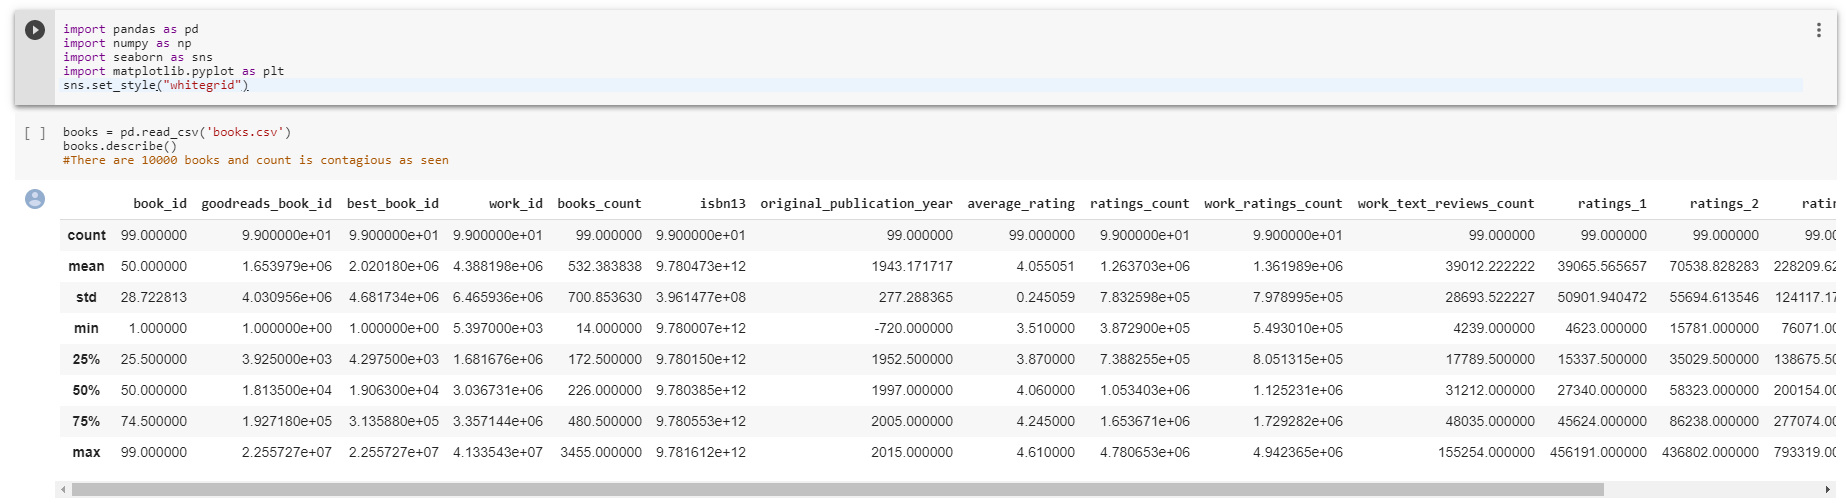
\includegraphics[scale= 0.30]{./Imagenes/captura1.png}
\end {center}

\begin {center}
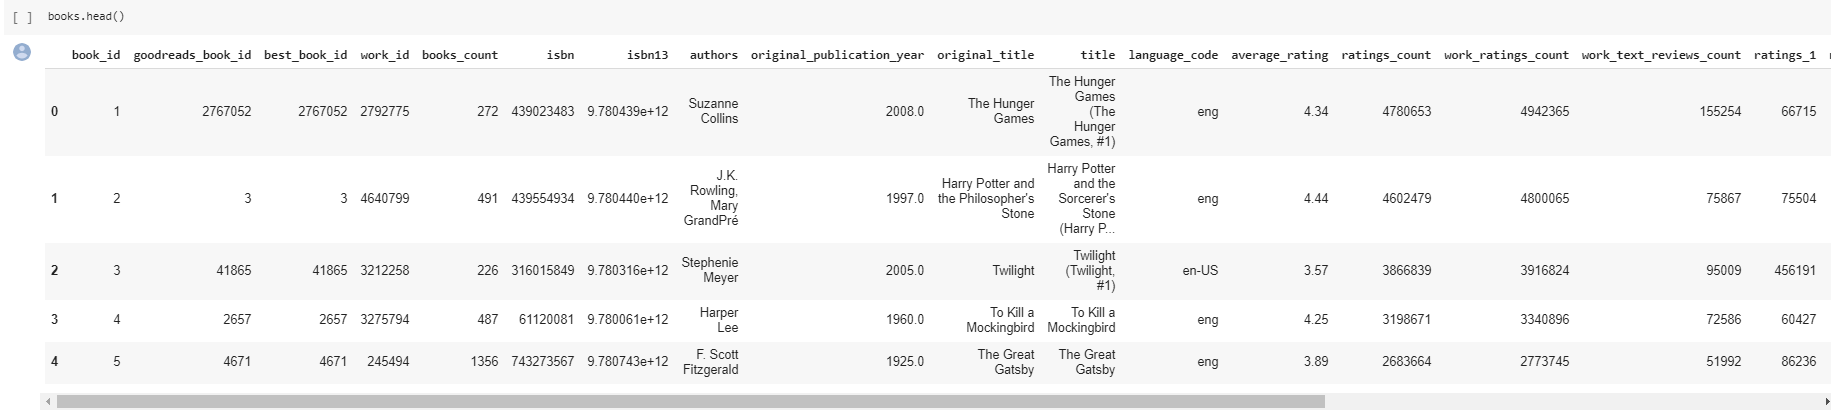
\includegraphics[scale= 0.30]{./Imagenes/captura3.png}
\end {center}

\item Nombre  de los autores del archivo book.csv


\begin {center}
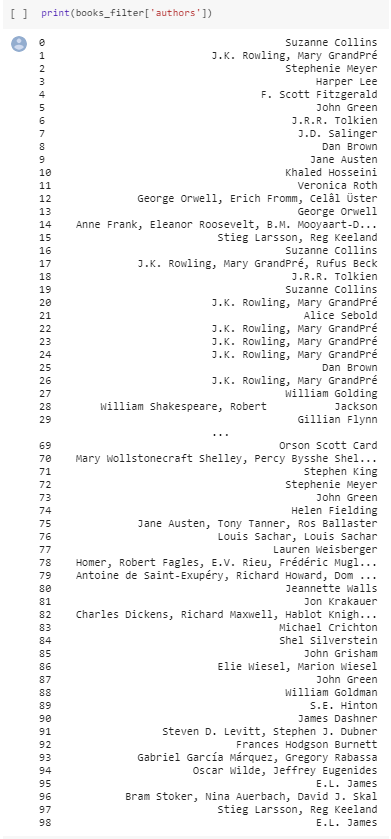
\includegraphics[scale= 0.81]{./Imagenes/captura5.png}
\end {center}

\item  Titulos de los libros del archivo book.csv


\begin {center}
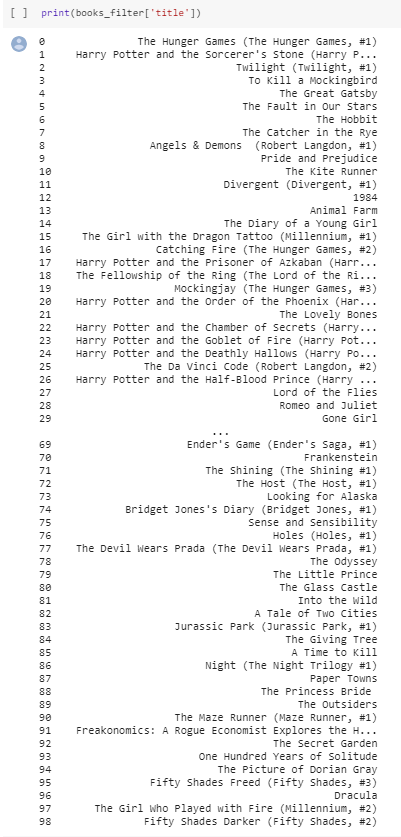
\includegraphics[scale= 0.81]{./Imagenes/captura4.png}
\end {center}


\item Consultas de Mejores Libros

\begin {center}
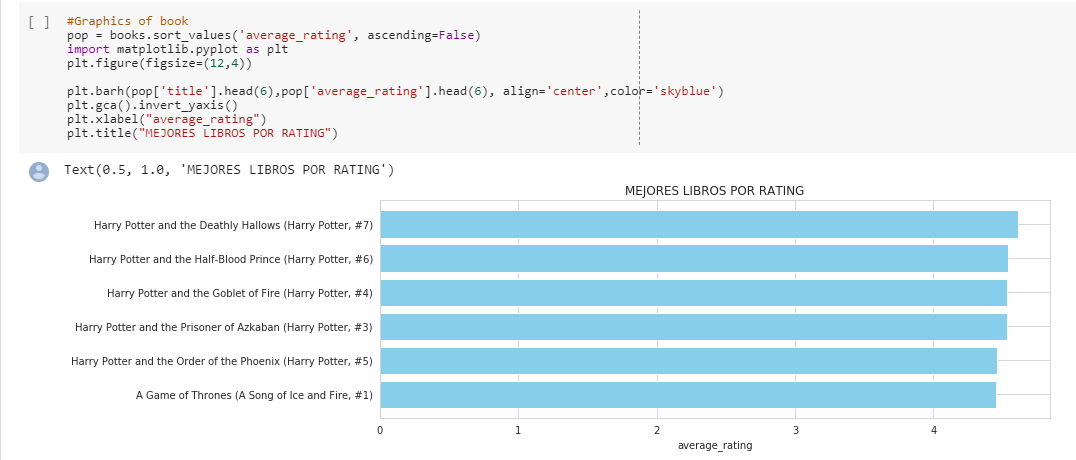
\includegraphics[scale= 0.50]{./Imagenes/captura2.png}
\end {center}


\item Consultas de Mejores Libros por Autor 

Este objetivo se hace necesario para poder iniciar una valoracion de los autores.

\begin {center}
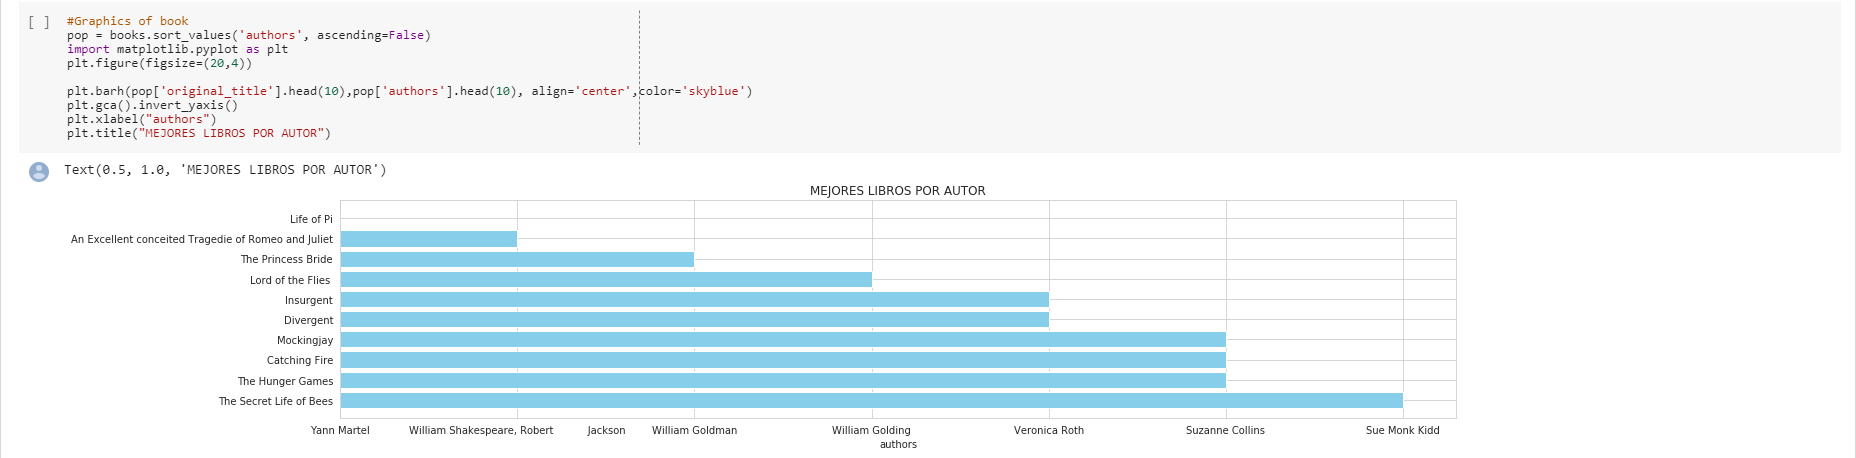
\includegraphics[scale= 0.40]{./Imagenes/libros-autor.png}
\end {center}


\item Consultas de Mejores Libros por Rating 1

Este objetivo se hace necesario para poder iniciar una valoracion de los libros.

\begin {center}
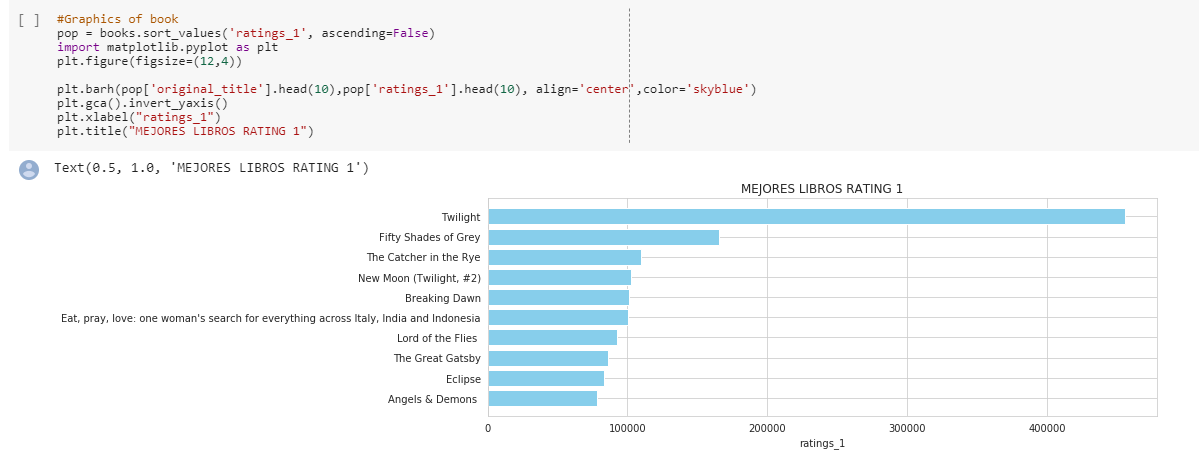
\includegraphics[scale= 0.50]{./Imagenes/libros.png}
\end {center}


\end{itemize}


\section{Conclusion}
Un sistema de recomendaciones es mucho más que un algoritmo o un filtro que selecciona productos con más o menos acierto. Podemos dividir un recomendador en 4 partes: la base de conocimiento (la información, los datos), el procesamiento de la base de conocimientos (tecnología, algoritmos, filtros), la analítica y control de negocio (medir todo, estrategia de negocio) y finalmente el interface del usuario.

Para terminar, y ya que estamos en un mundo de datos, pongamos un peso a cada una de ellas:
\begin{itemize}
	\item Base de conocimiento – 25%\\
	\item Procesamiento de la base de conocimientos – 5%\\
	\item Analítica y control de negocio – 20%\\
	\item Interface del usuario – 50%\\
\end{itemize}

Evalúa tu entorno, tu producto, tu negocio, la calidad y cantidad de tus datos, el comportamiento de tus clientes y construye el recomendador adecuado a tus necesidades. Si deseas conocer más sobre el tema, no dudes en ponerte en contacto con nosotros

	

	
	
	\newpage
	
		%ESTILO
	   \bibliography{BIBLIOGRAFIA}		%ARCHIVO .bib
	   \begin{thebibliography}{0}
              \bibitem{Ronald} http://blog.findemor.es/2018/02/sistemas-de-recomendacion-en-python/
	    \bibitem{Ronald} https://medium.com/datos-y-ciencia/construye-tu-primer-clasificador-de-deep-learning-con-tensorflow-ejemplo-de-razas-de-perros-ed218bb4df89	
 	    \bibitem{Angelo} https://platzi.com/blog/que-es-y-como-funciona-filtrado-colaborativo/
                 \bibitem{Juan} http://tdan.com/data-warehouse-design-inmon-versus-kimball/20300
                  \bibitem{Jhordy} https://programacionpython80889555.wordpress.com/2019/02/19/representacion-grafica-de-datos-en-python-con-matplotlib-grafico-de-barras/
                  \bibitem{Jhordy} http://www.iac.es/sieinvens/python-course/source/matplotlib.html
                    \bibitem{Brandon} https://www.iebschool.com/blog/filtrado-colaborativo-sirve-e-commerce/
                   \bibitem{Brandon} https://noticias.universia.net.mx/ciencia-nn-tt/noticia/2004/11/14/115495/como-funciona-filtro-contenido.html

         \end{thebibliography}
	
\end{document}

%%
%% End of file `elsarticle-template-1-num.tex'.
